%!TEX root = ../my_thesis.tex
\graphicspath{{main/chapter2/fig/}}

\chapter{Algorithms and Efficient Methods of Receiver}

\section{Strategy for Optimizations}

\subsection{Algorithmic Simplifications}

\subsection{Memory Data Layer}

\subsection{Quantification}

\subsection{Vectorization~\cite{Cassagne2018}}

\begin{itemize}
  \item \xmark~le temps d'exécution d'une tâche peut varier entre quelques
        microsecondes et quelques milliseconde -> faible latence -> adapté à la
        vectorisation
  \item \xmark~expliquer les approches intra-trame et inter-trame pour faire du
        SIMD
  \item \cmark~\textbf{état de l'art wrapper SIMD}
  \item \cmark~portabilité (ARM to Xeon Phi)
\end{itemize}

Recent articles have proposed several optimized software decoders, corresponding
to different channel codes : LDPC codes~\cite{LeGal2015,LeGal2016}, polar
codes~\cite{Giard2016b,Sarkis2016,Cassagne2015c,Cassagne2016b}, turbo
codes~\cite{Zhang2012,Wu2013,Cassagne2016a}. All of these works show the
possibility to reach a good level of \textit{performance} by  making extensive
use of SIMD (Single Instruction Multiple Data) units. This is often achieved at
the price of a reduced \textit{flexibility}, by resorting to specific
intrinsics, or by making assumptions on the data types. However, these decoders
should be implemented in a single source code, in which the following parameters
could be changed at runtime: the channel code type, the decoding algorithm, the
number of decoding iterations, the data format, etc. Another important aspect is
the \textit{portability} of the source code on different hardwares (Intel x86,
Xeon KNL and ARM) and the possibility to use different instruction sets
(\verb|SSE|, \verb|AVX|, \verb|AVX-512|, \verb|NEON|). These three constraints
(performance, flexibility, portability) push towards the use of a SIMD library
that helps in the abstraction of the SIMD instruction sets, while still allowing
a fine grain tuning of performance.

We propose in this thesis a new \Cxx SIMD wrapper, covering the needs in terms
of expressiveness and of performance for the channel codes. Our contributions
are:
\begin{itemize}
  \item A portable and high performance  \Cxx SIMD wrapper called \MIPP, for
        \verb|SSE|, \verb|AVX|, \verb|AVX-512| and \verb|NEON| instruction sets;
  \item An implementation of several channel codes with this wrapper. We
        present the main advantages of \MIPP in this context;
  \item A comparison with other state-of-the-art SIMD
        wrappers on a Mandelbrot code, demonstrating that the code based on
        \MIPP has similar performance as hand-written intrinsics.
\end{itemize}
\MIPP programming model is not too far from intrinsics, allowing a good control
on performance, but still provides an abstraction on the basic types used in
vectors (ranging from double to byte) and complex operations (parametric
reductions, log, exponential, ...).

The \longMIPP library (\MIPP) is a portable wrapper for SIMD intrinsics written
in the \Cxx language. It relies on \Cxx compile-time template specialization
techniques to replace supported generic functions with inline calls to their
intrinsics counterpart, for a given instruction set. While \MIPP is mostly
written in \Cxy{98}, it still requires \Cxy{11}-compliant compiler due to the
use of convenient features such as the \verb|auto| and \verb|using| keywords.
\MIPP is Open-source (under the MIT license) and the full code is available on
GitHub\footnote{\MIPP source code: \url{https://github.com/aff3ct/MIPP}}.

\MIPP provides two application programming interface levels. The
\emph{Low Level Interface} (low) implements a basic, thin abstraction layer on
top of the intrinsics. The \emph{Medium Level Interface} (med.), built on top of
\MIPP low, abstracts away more details to lessen the effort from the application
programmer by relying on object encapsulation and operator overloading.

\subsubsection{Low Level Interface}

\MIPP low is built around a unified \verb|mipp::reg| type that abstracts vector
registers. The vector register type represents hardware registers independently
of the data type of the vector elements. \MIPP uses the longest native vector
length available on the architecture. This design choice preserves programmer
flexibility, for instance in situations such as mixing fixed-point and
floating-point operations. \MIPP also defines a \emph{mask} register type
\verb|mipp::msk|, which either directly maps to real hardware masks on
instruction sets that support it (such as AVX-512), or to simple vector
registers otherwise.

\MIPP low then defines a set of functions working with \verb|mipp::reg| and
\verb|mipp::msk|, organized into eight families: memory accesses, shuffles,
bitwise boolean arithmetic, integer operations, float. operations, mathematical
functions, reductions, and mask operations.

In the AVX-512 instruction set, one \textit{regular} vector operation plus one
masking operation can be performed in one CPU clock cycle. For instance, the
following instruction performs \verb|"m ? a+b : src"|, an addition and a masking
operation:
\mint{C++}|__m512 _mm512_mask_add_ps(__m512 src, __mmask16 m, __m512 a, __m512 b);|

\MIPP natively supports such operations with the \verb|mipp::mask| function. The
previous example becomes in \MIPP:
\mint{C++}|mipp::mask<float,mipp::add<float>>(m, src, a, b);|
For instruction sets without masking support, the \verb|mipp::mask| call is
expanded as an operation and a \verb|blend| instead.

\subsubsection{Medium Level Interface}

\begin{listing}[htp]
  \inputminted[frame=lines,linenos]{C++}{main/chapter2/src/vectorization/mipp_mli.cpp}
  \caption{Medium Level Interface encapsulation.}
  \label{lst:MLI}
\end{listing}

The \MIPP Medium Level Interface (\MIPP med.) provides additional expressiveness
to the programmer. \verb|mipp::reg| and \verb|mipp::msk| basic types are
encapsulated in \verb|mipp::Reg<T>| and \verb|mipp::Msk<N>| objects,
respectively. The \verb|T| and \verb|N| template parameters correspond to the
type and the number of elements inside the vector register and the mask
register, respectively. One can notice that in these register objects are typed,
unlike the \MIPP low register basic type. It avoids to write the type when a
\MIPP function is called. The function type can then be directly selected from
the parameter type. Listing~\ref{lst:MLI} illustrates the template-based
encapsulation, which enables \MIPP to override common arithmetic and comparison
operators.

\MIPP med. also simplifies register loading and initialization operations. The
constructor of the \verb|mipp::Reg| object will call the \verb|mipp::load|
function automatically. Thus, a load in \MIPP low:
\mint{C++}|mipp::reg a = mipp::load<float>(aligned_ptr);|
can be simplified into:
\mint{C++}|mipp::Reg<float> a = aligned_ptr;|
with \MIPP med. level. An initializer list
can be used with a \MIPP med. vector register:
\mint{C++}|mipp::Reg<float> a = {1.f, 2.f, 3.f, 4.f};|
Likewise, a scalar assigned to a vector sets all elements to
this value.

\subsubsection{Implementation Details}
\label{subsec:implem}

\MIPP targets \verb|SSE2|, \verb|SSE3|, \verb|SSSE3|, \verb|SSE4.1|,
\verb|SSE4.2|, \verb|AVX|, \verb|AVX2|, \verb|FMA3|, \verb|KNCI|,
\verb|AVX-512F| and \verb|AVX-512BW| instruction sets on x86 and related
architectures, as well as \verb|NEON|, \verb|NEONv2|, \verb|NEON64| and
\verb|NEON64v2| on ARM. It can easily be extended to other instruction sets.

\MIPP selects the most recent instruction set available at compile time. For
instance, a code compiled with the \verb|-march=avx| flag of the GNU GCC
compiler uses \verb|AVX| instructions even if the architecture supports
\verb|SSE| as well. The vector register size is determined by the instruction
set and the data type. A dedicated function returns the number of elements in a
\MIPP register:
\mint{C++}|constexpr int n = mipp::nElmtsPerRegister<T>();|
A shortened version is also defined as: \verb|mipp::N<T>()|. Whenever
vectorization takes place in loops, \MIPP's philosophy is to change the stride
of the loop from one to the size of registers. The stride can be statically
determined with the \verb|mipp::N<T>()| function.
If the loop size is not a multiple of the registers size, 1) a sequential tail
loop can be implemented to compute the remaining elements, 2) the padding
technique can be implemented to force the loop size to be a multiple of the
vector registers.

When the instruction set cannot be determined, \MIPP med. falls back on
sequential instructions. In this case, \MIPP does not use any intrinsic anymore.
However, the compiler vectorizer still remains effective. This mode can also be
selected by the programmer with the \verb|MIPP_NO_INTRINSICS| macro.

\MIPP supports the following data types: \verb|double|, \verb|float|,
\verb|int64_t|, \verb|int32_t|, \verb|int16_t| and \verb|int8_t|. It also
supplies an aligned memory allocator, to be used with types such as the
\verb|std::vector<T,A>| vector container from the \Cxx standard library (where
\verb|T| is the vector element type and \verb|A| the allocator). The alignment
requirements are not guaranteed by the default \Cxx memory allocator. The \MIPP
memory allocator can be used as follows:
\mint{C++}|std::vector<T,mipp::allocator> aligned_data;|
and shortened like this: \verb|mipp::vector<T>|.

\MIPP comes with a comprehensive unitary test suite to validate new instruction
set ports and new feature implementations. It has successfully been tested with
the following minimum compiler versions: \verb|g++-4.8|, \verb|clang++-3.6|,
\verb|icpc15| and \verb|msvc14.0|.

\MIPP implements a generic reduction operator based on a reduction tree, which
would be tedious to write by the application programmer, due to the sequence of
heterogeneous shuffle instructions it implies. The computational complexity of
this algorithm is $O(\log_2(N))$, with $N$ the number of elements in a register.
It can operate on \verb|mipp::reg|, \verb|mipp::Reg<T>| and
\verb|std::vector<T>|. It can also work on dynamically allocated arrays,
provided the length of the array is a multiple of the vector register size.
Since the function passed to the reduction operator is resolved at the compile
time, the code remains efficient. Any function with the following prototype can
be used as the reduction function:
\mint{C++}|mipp::Reg<T> func(mipp::Reg<T>, mipp::Reg<T>);|
E.g., the code below computes the smallest element in a register:
\begin{minted}{C++}
mipp::Reg<float> r = {4.f, 2.f, 1.f, 3.f};
float min = mipp::Reduction<mipp::min>::sapply(r);
\end{minted}
The \verb|min| scalar variable will be assigned \verb|1.f| as the result. For
convenience, a set of functions is predefined, based on this generic reduction
feature: \verb|hadd|, \verb|hsub|, \verb|hmul| and \verb|hdiv|.

\subsubsection{Related Works}

Many SIMD programming solutions have been surveyed in~\cite{Pohl2016} to take
advantage of modern instruction sets. The existing alternatives can be
decomposed into three main models: 1)~intrinsics or assembly code; 2)~dedicated
language; and 3)~dedicated library. The intrinsics or assembly approaches are
non-portable, low-level solutions which target specific architectures. They
offer maximum control to take advantage of instruction set specificities, and to
fine tune register usage. However, it is quite difficult to develop and maintain
a low-level code in the long run. Some languages have been designed to provide
programmers with SIMD programming constructs. Many of them are based on general
purpose languages extended with some kinds of annotation mechanism (e.g.
pragmas) such as OpenMP~\cite{OpenMP2013}, Cilk Plus~\cite{Robison2013} or
ispc~\cite{Pharr2012}. They offer higher expressiveness, better portability and
generally more readable code, at the expense of less programmer control, and
vectorization performance. More specialized languages, such as
OpenCL~\cite{Howes2015}, enable the programmer to retain more control, as the
counterpart of writing some more specific code.
In this paper, the focus is given to the library approach since we want to
maximize performance, maximize portability and deal with existing \Cxx codes. In
order to let the compiler inline library calls, which is critical for the
intended SIMD programming model purpose, such library are usually header-only.
Thus, we refer to them as \textit{wrappers} instead of \textit{libraries}.

\paragraph{\Cxx SIMD Wrappers}

\begin{table*}[htp]
  \renewcommand{\arraystretch}{0.95}
  \tabcolsep=6pt
  \centering
  \caption{Comparison of various SIMD wrappers.}
  \label{tab:comp}
  {\small\resizebox{\linewidth}{!}{
  \begin{tabular}{|r|r|r|r|r||c|c|c|c|c||c|c|c|c|c|c||c|c|c|}
  \hline
  \multicolumn{5}{|c||}{\multirow{2}{*}{\textbf{General Information}}}                                                               & \multicolumn{5}{c||}{\multirow{2}{*}{\textbf{Instruction Set}}}                                                                & \multicolumn{6}{c||}{\multirow{2}{*}{\textbf{Data Type}}}                    & \multicolumn{3}{c|}{\multirow{2}{*}{\textbf{Features}}} \\
  \multicolumn{5}{|c||}{}                                                                                                            & \multicolumn{5}{c||}{}                                                                                                         & \multicolumn{6}{c||}{}                                                       & \multicolumn{3}{c|}{}                                  \\ \hline
  \multicolumn{2}{|r|}{\textbf{Name}}                                      & \textbf{Ref.}       & \textbf{Start} & \textbf{License} & \textbf{\texttt{SSE}} & \textbf{\texttt{AVX}} & \textbf{\texttt{AVX-512}} & \textbf{\texttt{NEON}} & \textbf{\texttt{AltiVec}} & \multicolumn{2}{c|}{\textbf{Float}} & \multicolumn{4}{c||}{\textbf{Integer}} & \textbf{Math}  & \textbf{\Cxx}      & \textbf{Test}    \\ \cline{11-16}
  \multicolumn{2}{|r|}{}                                                   &                     & \textbf{Year}  &                  & 128-bit               & 256-bit               & 512-bit                   & 128-bit                & 128-bit                   & 64      & 32                        & 64     & 32     & 16     & 8           & \textbf{Func.} & \textbf{Technique} & \textbf{Suite}   \\ \hline \hline
  \multirow{8}{*}{\rotatebox[origin=c]{90}{\textbf{Library}}} & \MIPP      & $-$                 & 2013           & MIT              & \cmark                & \cmark                & \cmark                    & \cmark                 & \xmark                    & \cmark  & \cmark                    & \cmark & \cmark & \cmark & \cmark      & \cmark         & Op. overload.      & \cmark           \\ \cline{2-19}
                                                              & \VCL       & \cite{Fog}          & 2012           & GNU GPL          & \cmark                & \cmark                & \cmark                    & \xmark                 & \xmark                    & \cmark  & \cmark                    & \cmark & \cmark & \cmark & \cmark      & \cmark         & Op. overload.      & \textbf{N/A}     \\ \cline{2-19}
                                                              & \simdpp    & \cite{Kanapickas}   & 2013           & Boost Software   & \cmark                & \cmark                & \cmark                    & \cmark                 & \cmark                    & \cmark  & \cmark                    & \cmark & \cmark & \cmark & \cmark      & \xmark         & Expr. templ.       & \cmark           \\ \cline{2-19}
                                                              & \TSIMD     & \cite{Moller2016}   & 2016           & Open-source      & \cmark                & \cmark                & \xmark                    & \cmark                 & \xmark                    & \xmark  & \cmark                    & \xmark & \cmark & \cmark & \cmark      & \xmark         & Op. overload.      & \textbf{N/A}     \\ \cline{2-19}
                                                              & \Vc        & \cite{Kretz2012}    & 2012           & BSD-3-Clause     & \cmark                & \cmark                & \xmark                    & \xmark                 & \xmark                    & \cmark  & \cmark                    & \cmark & \cmark & \cmark & \xmark      & \cmark         & Op. overload.      & \cmark           \\ \cline{2-19}
                                                              & \xsimd     & \cite{Mabille}      & 2014           & BSD-3-Clause     & \cmark                & \cmark                & \xmark                    & \xmark                 & \xmark                    & \cmark  & \cmark                    & \cmark & \cmark & \xmark & \xmark      & \cmark         & Op. overload.      & \textbf{N/A}     \\ \cline{2-19}
                                                              & \BoostSIMD & \cite{Esterie2012}  & 2012           & Boost Software   & \cmark                & \xmark                & \xmark                    & \xmark                 & \xmark                    & \cmark  & \cmark                    & \cmark & \cmark & \cmark & \cmark      & \cmark         & Expr. templ.       & \cmark           \\ \cline{2-19}
                                                              & \bSIMD     & \cite{Esterie2012a} & 2017           & Non-free         & \cmark                & \cmark                & \cmark                    & \cmark                 & \cmark                    & \cmark  & \cmark                    & \cmark & \cmark & \cmark & \cmark      & \cmark         & Expr. templ.       & \cmark           \\ \hline
  \end{tabular}
  }}
\end{table*}

\begin{figure*}[htp]
\centering
\includegraphics[width=0.90\textwidth]{vectorization/mandelbrot_speedup}
\caption{Speedups over the Mandelbrot naive auto-vectorized implementation}
\label{fig:fractal}
\end{figure*}

Table~\ref{tab:comp} compares various SIMD wrappers. It aims to present an
overview of some prominent solutions, though it is by no means exhaustive due to
the richness of the SIMD wrapper landscape. Some of the wrappers presented, such
as \MIPP, \Vc, \BoostSIMD, \VCL and \TSIMD, have been designed in an academic
research context. Some others, \simdpp and \xsimd, appear to be standalone
development efforts by individual programmers or maintainers. Proprietary,
closed-source solutions also exist on the market, such as \bSIMD, which is an
extended version of \BoostSIMD, or the commercial version of \VCL. The
\textit{Instruction Set} column is broken up into five families among the most
widely available on the market: \verb|NEON|, \verb|SSE|, \verb|AVX|,
\verb|AVX-512| and \verb|AltiVec|. For the sake of conciseness, we choose not to
list all the instruction sets ``sub-variants'' (such as \verb|SSE2|,
\verb|SSE3|, etc). \simdpp et \bSIMD propose the most comprehensive instruction
set compatibility. At the other end of the range, \xsimd and \BoostSIMD only
support Intel SIMD instruction sets. The \textit{Data Type} column of the table
summarizes the supported vector element types and precisions. In their public
version, and at the time of writing, \Vc does not support 8-bit integers, \xsimd
does not support 8-bit and 16-bit integers and \TSIMD does not support 64-bit
data types, to the best of our knowledge. The \textit{Features} column
highlights some additional characteristics. The \textit{Math Func.}~ column
indicates which wrapper supports additional mathematical sub-routines, not
necessarily available as native CPU instructions (exponential, logarithm,
trigonometric functions for instance), and required by algorithms such as the
Box-Muller Transform (see Section~\ref{subsec:bmt}). The \textit{\Cxx Technique}
column indicates whether the wrapper is designed as an expression template
framework, or whether it relies on operator overloading techniques. The
expression template feature is a powerful technique to automatically drive the
rewriting of whole arithmetic expressions into SIMD hardware instructions or
instruction sequences. For instance if the user writes \verb|d = a * b + c|, the
wrapper can automatically match a \emph{fused multiply and add} instruction
(FMA). \BoostSIMD and \bSIMD extensively use this
technique~\cite{Esterie2012,Esterie2012a}. The drawbacks are that the source
code complexity of the wrapper is dramatically increased. \BoostSIMD and \bSIMD
have a dependency on the Boost framework to build, and currently available \Cxx
compilers produce huge amounts of arcane error messages at the slightest mistake
in the end user program. For these reasons, we decided not to base \MIPP on the
expression template technique. As mentioned in Section~\ref{subsec:implem},
maintaining SIMD wrappers, and porting them to new instruction sets is error
prone by nature, due to the large number of routines, cryptic intrinsics names,
and specific instruction set details. A comprehensive testing suite is therefore
critical to validate new development, optimizations and ports on new instruction
sets. This is why \MIPP, as well as \Vc, \BoostSIMD, \simdpp and \bSIMD come
with their own test suites. We have not found similar test suites in the
software distributions of \VCL, \xsimd and \TSIMD; however, test suites might be
in use internally, within the development teams of these wrappers.

\paragraph{Qualitative and Quantitative Comparisons}

We now compare \MIPP with the open-source wrappers presented above, both
qualitatively for our error correction code purpose, and quantitatively on a
well known benchmark the computation of the Mandelbrot set, to prevent as much
as possible the risk of unfairness of the port on each wrapper. This problem is
compute-bound. The chosen implementation relies on a floating-point
representation (available online\footnote{Mandelbrot set source code:
\url{https://gitlab.inria.fr/acassagn/mandelbrot}}). Figure~\ref{fig:fractal}
presents the speedups obtained on various instruction sets. \verb|SSE| stands
for \verb|SSE4.2|, \verb|NEON| stands for \verb|NEONv2| (includes the FMA
instructions), \verb|AVX| stands for \verb|AVX2+FMA3| and \verb|AVX-512| stands
for \verb|AVX-512F| (with FMA instructions). The \verb|FMA| benefit ranges from
17\% (\verb|AVX2|) to 26\% (\verb|AVX-512|). An SIMD with intrinsics version has
been hand-coded for each specific instruction set. The intrinsics version is
considered the ``\emph{golden}'' model.

\textbf{\BoostSIMD} only supports the \verb|SSE| instruction set, even when the
code is compiled with one of the \verb|AVX| or \verb|AVX-512| flags. It is
insufficient for our channel coding processing purpose. The \BoostSIMD wrapper
performance results that were obtained are disappointing. The sequential
Mandelbrot kernel does an early exit in the innermost loop, as soon as the
divergence of the sequence is detected for the input coordinates. We were unable
to SIMDize this early termination with \BoostSIMD, because the
\verb|boost::simd::any| function was not available in the GitHub repository at
the time of writing.
\textbf{\xsimd} achieves performance close to the intrinsic version in
\verb|SSE| and \verb|AVX|. However, it currently lacks \verb|NEON| and
\verb|AVX-512| support. Moreover, it does not support small 8-bit and 16-bit
integers, needed for Successive Cancellation decoders (see
Section~\ref{subsec:polar}).
\textbf{\Vc} is one of the earliest developed SIMD \Cxx wrapper. We used
Branch~1.3 for the performance measurements, the latest stable branch at this
time. \Vc includes a lot of of features compared to the other wrappers; but it
lacks support for \verb|NEON| and \verb|AVX-512| (which are currently being
developed). Performance results are on par with the best contenders for
\verb|AVX|. However, a slowdown is observed for \verb|SSE|. Note: For
\verb|AVX-512|, since the support is not yet available in the stable version, we
used the capability of \Vc to generate \verb|AVX2| code in order to produce the
sample points for \verb|AVX-512| series. The results are likely to improve once
the full \verb|AVX-512| support is release in a subsequent stable version.
\textbf{\TSIMD} is a wrapper primarily designed for image processing purpose.
It performs well in 32-bit \verb|NEON|, \verb|SSE| and \verb|AVX| but it lacks
from \verb|AVX-512|. Support of the 64-bit types is not planed since it is not
useful in traditional image computations.
\textbf{\simdpp} supports an impressive number of instruction sets. This may
explain why it does not support mathematical functions so far. It matches the
performance of the other wrappers for \verb|NEON| and \verb|SSE|, but falls
behind for \verb|AVX|, and even more for \verb|AVX-512|.
\textbf{\VCL} is a high performance wrapper and perhaps the most feature rich
for x86 SIMD at this time. It gives a lot of control to the developer and it is
well documented. The obtained performance are on the same level as hand-written
intrinsics. However, it is not yet available on \verb|NEON|.
For \MIPP we have tested both the lower-level programming
interface and the medium-level programming interface of our \MIPP wrapper,
mainly to detect potential overheads when using the medium level interface
instead of the lower one. The obtained results do not show any performance
penalties when using \MIPP medium level interface. The obtained speedups are
close to the intrinsics version.

\MIPP corresponds to a programming model close to the intrinsics, with some
adaptation to architectures. Still, a high performance code requires that the
developer knows how to decompose efficiently some computation with the SIMD
instructions. Between \verb|AVX-512| and \verb|SSE| or \verb|NEON| for instance,
several implementations of the same code are possible. \MIPP offers to the
programmer the control on the intrinsics taken and ensures portability.

\section{Polar Decoders~\cite{Cassagne2015c,Cassagne2016b,Leonardon2019}}

\subsection{Fast Implementations}

\subsubsection{Related Works}

HoF polar: \url{http://aff3ct.github.io/hof_polar.html}

\subsubsection{Successive Cancellation Algorithm}

\subsubsection{Successive Cancellation List Algorithm}

\subsubsection{Tree Pruning Strategies}

\begin{itemize}
  \item élagage
\end{itemize}

\subsubsection{Vectorization Strategies}

\begin{itemize}
  \item polar API
  \item inter/intra-SIMD
\end{itemize}

\subsubsection{Unrolling}

\begin{itemize}
  \item décodeurs générique (pas déroulé)
  \item déroulage d'arbre
\end{itemize}

\subsubsection{Evaluations}

\begin{itemize}
  \item 32-bit, 16-bit, 8-bit
  \item consommation énergétique ARM/x86
\end{itemize}

\subsection{Generic Kernels and Multi-Kernel}

\subsubsection{Related Works}

\subsubsection{Others}

\begin{itemize}
  \item factorisation automatique de kernels et génération du code source associé
  \item décodeurs multi-kernels génériques SC, SCL, CA-SCL et ASCL (non systématique et systématique)
\end{itemize}

\section{Turbo Decoders~\cite{Cassagne2016a}}

\subsection{Related Works}

HoF turbo: \url{http://aff3ct.github.io/hof_turbo.html}

\subsection{Maximum A Posteriori Algorithm}

\begin{itemize}
  \item décodeur Turbo LTE (3G/4G)
  \item treillis
\end{itemize}

\subsection{Vectorization Strategies}

\begin{itemize}
  \item inter-SIMD
  \item décodeur inter- et intra-SIMD LTE à faible latence
\end{itemize}

\subsection{Evaluations}

\begin{itemize}
  \item 32-bit, 16-bit, 8-bit
\end{itemize}

\section{LDPC Decoders}

\subsection{Related Works}

HoF LDPC: \url{http://aff3ct.github.io/hof_ldpc.html}

\subsection{BP Algorithms}

\begin{itemize}
  \item graphe biparti
\end{itemize}

LDPC codes is a family of channel codes that is well spread in current digital
communication systems. They have been chosen in many communication standards
(Wifi, WiMAX, DVB-S2, 10Gbps Ethernet, etc.). They were also selected for the
future 5G standard data transport.

\begin{figure}[htp]
  \centering
  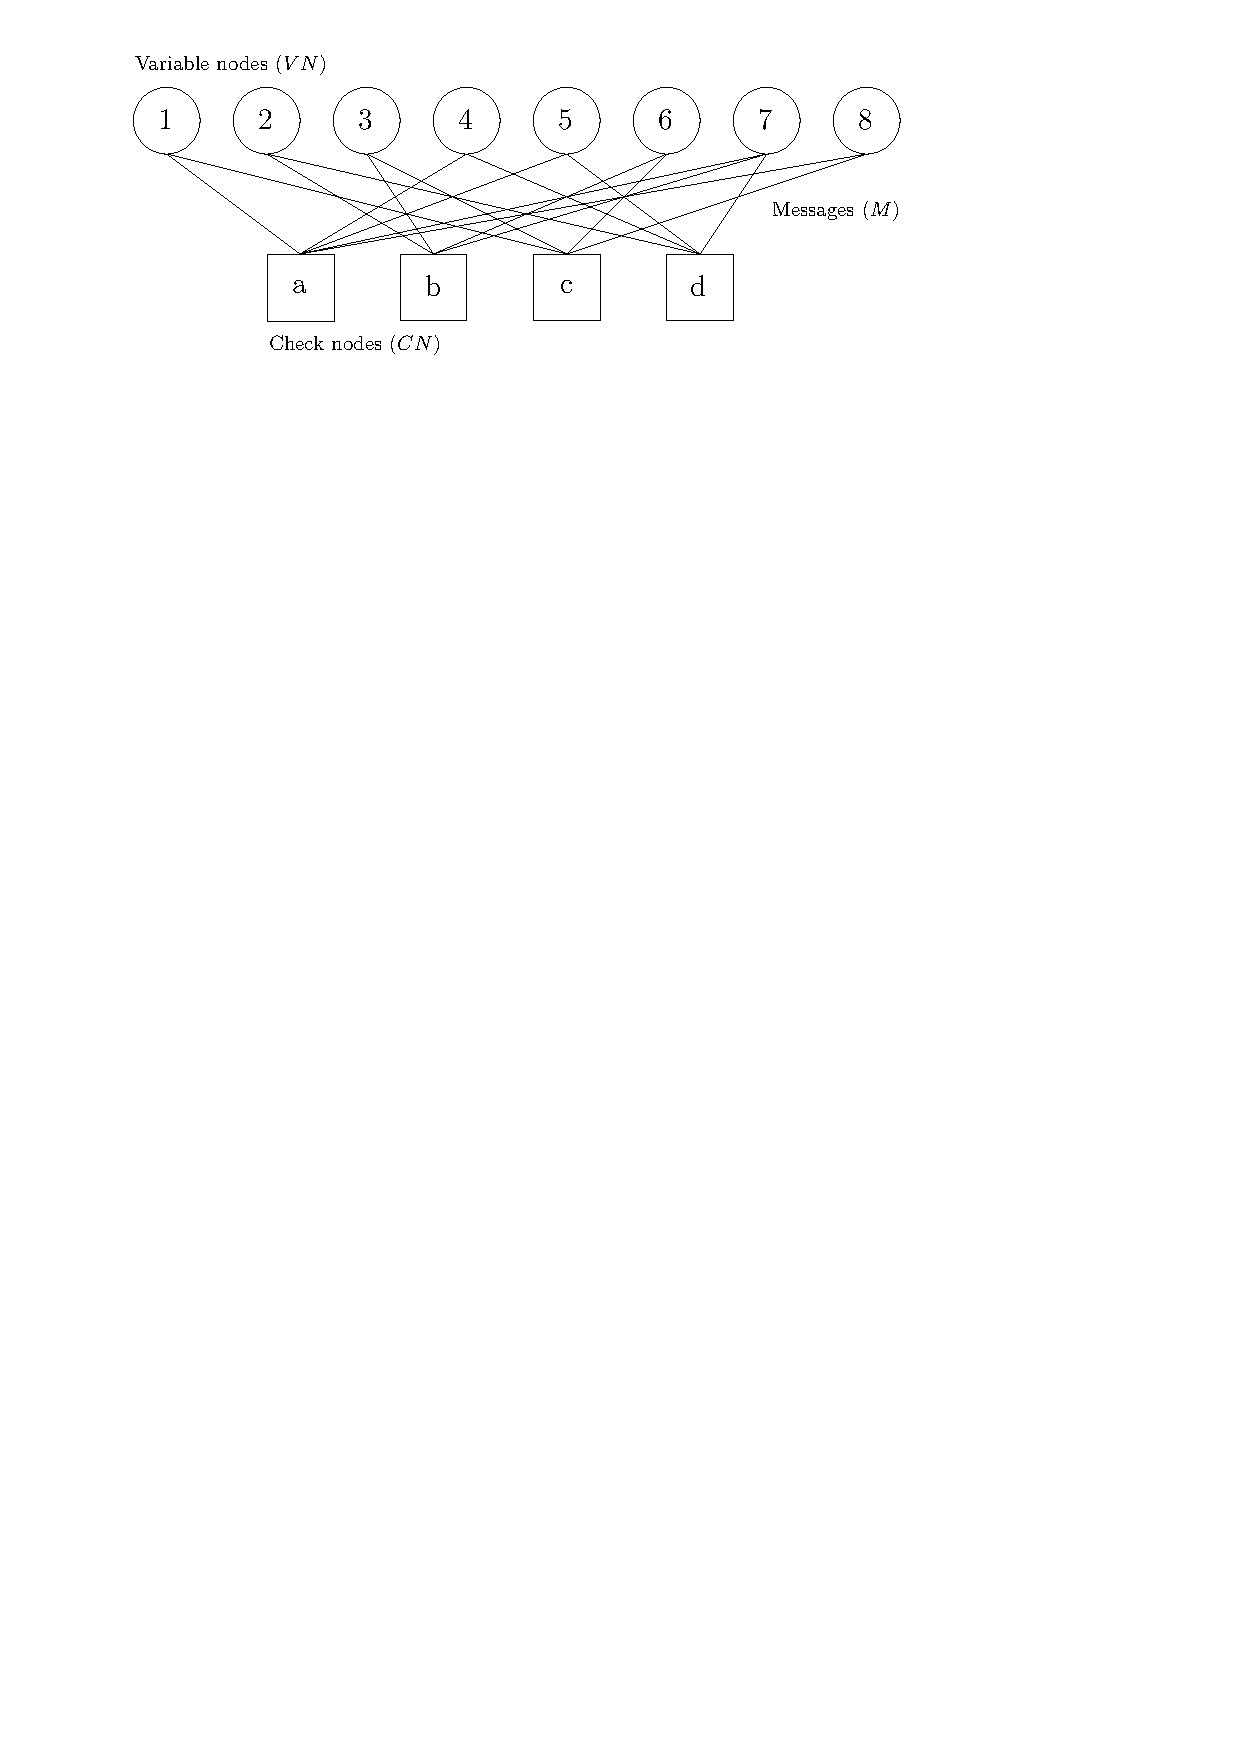
\includegraphics[width=0.60\textwidth]{ldpc/ldpc_tanner_graph}
  \caption{Tanner graph of a simple parity check $H$ matrix}
  \label{fig:LDPC}
\end{figure}

In this section the Min-Sum decoder for LDPC codes is presented. As shown in
Figure~\ref{fig:LDPC}, an LDPC code can be represented in the form of a Tanner
graph. The circles, denoted as variable nodes, represent the LLRs (the noisy
estimation of the bits in the received frames). The squares, denoted as parity
check nodes, represent the parity constraints that the variable nodes have to
verify. For instance, the check node $a$ ($CN_a$) is connected to the variable
nodes $1$, $4$, $5$, $7$ and $8$ ($VN_1, VN_4, VN_5, VN_7, VN_8$). It means that
the corresponding bits $U_1, U_4, U_5, U_7, U_8$ have to respect a parity
constraint: $U_1 \oplus U_4 \oplus U_5 \oplus U_7 \oplus U_8 = 0$. A codeword is
valid only if it respects all the parity constraints defined by the check nodes.
The LDPC code can be also represented by a \textit{parity check matrix}:
{ \begin{equation*}
H =
\begin{bmatrix}
  1&0&0&1&1&0&1&1\\
  0&1&1&0&0&1&1&0\\
  1&0&1&0&0&1&0&1\\
  0&1&0&1&1&0&1&0
\end{bmatrix}.
\end{equation*}
}
The Min-Sum decoder is an iterative message passing algorithm based on the
Tanner graph representation. Probabilistic messages ($M$) are exchanged between
the variable nodes and check nodes iteratively. Variable nodes and check nodes
apply an \textit{update rule} to compute the outgoing messages from the incoming
messages. In this section, the Min-Sum update rule is considered as well as an
horizontal layered scheduling. The original version of the Min-Sum algorithm
works on floating-point values, but it has been shown that fixed-point
simplifications have very similar decoding performance. Moreover, a fixed-point
representation enables to pack more elements into SIMD registers.

\subsection{Generic Implementation}

\begin{itemize}
  \item décodeurs génériques (BP-flooding/HL/VL) sur les "update nodes"
\end{itemize}

\subsection{Vectorization Strategies}

\begin{itemize}
  \item versions séquentielles et inter-SIMD
\end{itemize}

Listing~\ref{lst:LDPC} shows a 16-bit fixed-point LDPC decoder. This decoder
works on several frames at once. Each element of the SIMD registers corresponds
to an element of a specific frame. This approach is called the
\textit{inter-frame} vectorization. This strategy maximizes decoder throughput
at the expense of latency. Notice that the data type can be switched from
\verb|int16_t| to \verb|int8_t|, \verb|int32_t|, \verb|float| or \verb|double|.
This \MIPP feature is important for digital communication: adapting the data
type without changing the source code enables to address varying constraints
with a single source code.

\begin{listing}[htp]
  \inputminted[frame=lines,linenos]{C++}{main/chapter2/src/ldpc/bp_min_sum.cpp}
  \caption{LDPC decoder implementation with \MIPP.}
  \label{lst:LDPC}
\end{listing}

\subsection{Evaluations}

\begin{itemize}
  \item 32-bit, 16-bit
\end{itemize}

\begin{table}[htp]
  \tabcolsep=6pt
  \centering
  \caption{LDPC decoder speedups with \MIPP.}
  \label{tab:sp_ldpc}
  {\small
  \begin{tabular}{r|r|r|r}
                      & \textbf{\texttt{NEON}} & \textbf{\texttt{SSE}} & \textbf{\texttt{AVX}} \\ \hline
  \textbf{SIMD size}  & 8                      & 8                     & 16                    \\ \hline
  \textbf{T/P} (Mb/s) & 8.3                    & 30.3                  & 53.2                  \\ \hline
  \textbf{Speedup}    & $\times 9.7$           & $\times 8.8$          & $\times 15.2$         \\
  \end{tabular}
  }
\end{table}

Table~\ref{tab:sp_ldpc} presents speedups obtained with \MIPP. Ten iterations
are performed and a stop criterion was implemented for the tests based on parity
check constraints (not shown in Listing~\ref{lst:LDPC}). The $H$ matrix comes
from the IEEE 802.3an standard (10Gbps Ethernet). Speedups are close to the SIMD
width. In \verb|NEON| and \verb|SSE| they even exceed it. Such result can be
explained by an optimized memory management compared to the sequential version
of the code.

\section{SCMA Demodulator~\cite{Ghaffari2019}}

\subsection{Related Works}

\subsection{Presentation}

\subsection{MPA Demodulation Algorithms}

\begin{itemize}
  \item démodulateur SCMA intra-SIMD
  \item proposition d'une approximation des calculs
\end{itemize}

\subsection{Evaluations}

\section{Discussion}
